\documentclass{article}
\usepackage[utf8]{inputenc}
\usepackage{titling}

% Header
\usepackage{fancyhdr}
\pagestyle{fancy}
\fancyhead{} % cancella tutti i campi
\fancyhead[R]{Progetto finale di Reti Logiche, A.A. 2021/2022}

% Immagini
\usepackage{graphicx}
\graphicspath{ {images/} }
\usepackage{float}

% Tabelle
\usepackage{tabu}
\usepackage{caption} 
\captionsetup[table]{skip=2pt}
\usepackage[table]{xcolor}
\usepackage{array}

% Liste
\usepackage{listings}
\usepackage{enumitem}
\setlist{topsep=2pt, itemsep=2pt, partopsep=2pt, parsep=2pt}

% Stack
\usepackage{tikz}
\usetikzlibrary{decorations.pathreplacing,calc}

\newcommand{\tikzmark}[2][-3pt]{\tikz[remember picture, overlay, baseline=-0.5ex]\node[#1](#2){};}

\tikzset{brace/.style={decorate, decoration={brace}},
 brace mirrored/.style={decorate, decoration={brace,mirror}},
}

\newcounter{brace}
\setcounter{brace}{0}
\newcommand{\drawbrace}[3][brace]{%
 \refstepcounter{brace}
 \tikz[remember picture, overlay]\draw[#1] (#2.center)--(#3.center)node[pos=0.5, name=brace-\thebrace]{};
}

\newcommand{\annote}[3][]{%
 \tikz[remember picture, overlay]\node[#1] at (#2) {#3};
}

% renew/new command
\renewcommand*\contentsname{Indice}
\renewcommand{\figurename}{Figura}
\renewcommand{\tablename}{Tabella}

\newcommand{\subtitle}[1]{%
  \posttitle{%
    \par\end{center}
    \begin{center}\large#1\end{center}
    \vskip0.5em}
}

% Titolo e info
\title{%
    \vspace{4cm}
    \huge Prova Finale (Progetto di Reti Logiche)}

\subtitle{%
    Politecnico di Milano \\
    Anno Accademico 2021/2022 \\
    \vspace{0,3cm}
    Prof. Fabio Salice
    \vspace{7cm}
    }

\author{%
  Filippo Fini\\
  \texttt{Codice persona XXXX, Matricola XXXX}
  \and
  Francesca Grimaldi\\
  \texttt{Codice persona XXXX, Matricola XXXX}
}

\date{}


\begin{document}

%%%%%%%%%%%%%%%%%%%%%%
%%%%%%% TITOLO %%%%%%%
%%%%%%%%%%%%%%%%%%%%%%
\begin{titlingpage}
\maketitle
\end{titlingpage}


%%%%%%%%%%%%%%%%%%%%%%
%%%%%%% INDICE %%%%%%%
%%%%%%%%%%%%%%%%%%%%%%
\tableofcontents


%%%%%%%%%%%%%%%%%%%%%%%%%%%%
%%%%%%% INTRODUZIONE %%%%%%%
%%%%%%%%%%%%%%%%%%%%%%%%%%%%
\newpage
\section{Introduzione}
Il Progetto finale di Reti Logiche (per l'A.A. 2021/2022) ha come scopo quello di descrivere in linguaggio VHDL e successivamente sintetizzare tramite VIVADO, un modulo hardware che applichi un codice convoluzionale con tasso di trasmissione $\frac{1}{2}$ ai dati letti da memoria, ed in seguito ne scriva il risultato nella memoria stessa.
Il componente deve dunque essere in grado di interfacciarsi correttamente con la memoria per la lettura e la scrittura dei dati, e di manipolare in modo appropriato l'input per ottenere un risultato che rispecchi la codifica convoluzionale.

\subsection{Descrizione generale}
Il modulo riceve in ingresso una sequenza di parole da 8 bit ciascuna. Ognuna di queste parole viene serializzata, ottenendo i singoli bit ai quali è poi applicato il codice convoluzionale $\frac{1}{2}$.
Come rappresentato nella Figura 1, ad ogni bit in ingresso ($U_{\small{k}}$) ne corrispondono 2 in uscita ($p_{\small{1k}}$,$p_{\small{2k}}$). 
\begin{figure}[H]
    \centering
    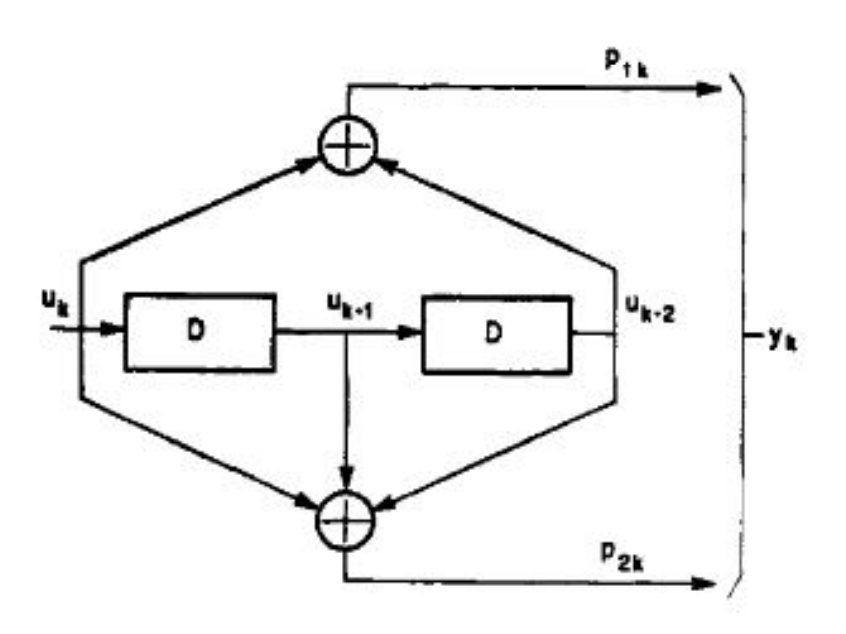
\includegraphics[width=0.5\textwidth]{cod_conv}
    \caption{Codificatore convoluzionale con tasso di trasmissione $\frac{1}{2}$}
    \label{fig:cod_conv}
\end{figure}
Tutti i bit di uscita vengono concatenati per generare un flusso continuo da 1 bit, e l'output finale sarà dato dalla parallelizzazione, su 8 bit, di questo flusso continuo.

\subsection{Serializzazione}
Il primo passo per l'applicazione dell'algoritmo è quello di serializzare l'input. Dato un flusso di W parole da 8 bit ciascuna, si vuole isolare volta per volta un bit.
Questo passo verrà ripetuto $8*W$ volte, e il bit dell'iterazione corrente andrà a costituire l'input per il convolutore.

\subsection{Codificatore convoluzionale}
Il convolutore è una macchina sequenziale sincrona, dotata di clock globale e segnale di reset, che ad un bit in ingresso ($U_{\small{k}}$) ne fa corrispondere 2 in uscita ($p_{\small{1k}}$, $p_{\small{2k}}$).
In Figura 2 è possibile vederne la rappresentazione come macchina di Mealy (notazione $U_{\small{k}}$/$p_{\small{1k}}$,$p_{\small{2k}}$).
\begin{figure}[H]
    \centering
    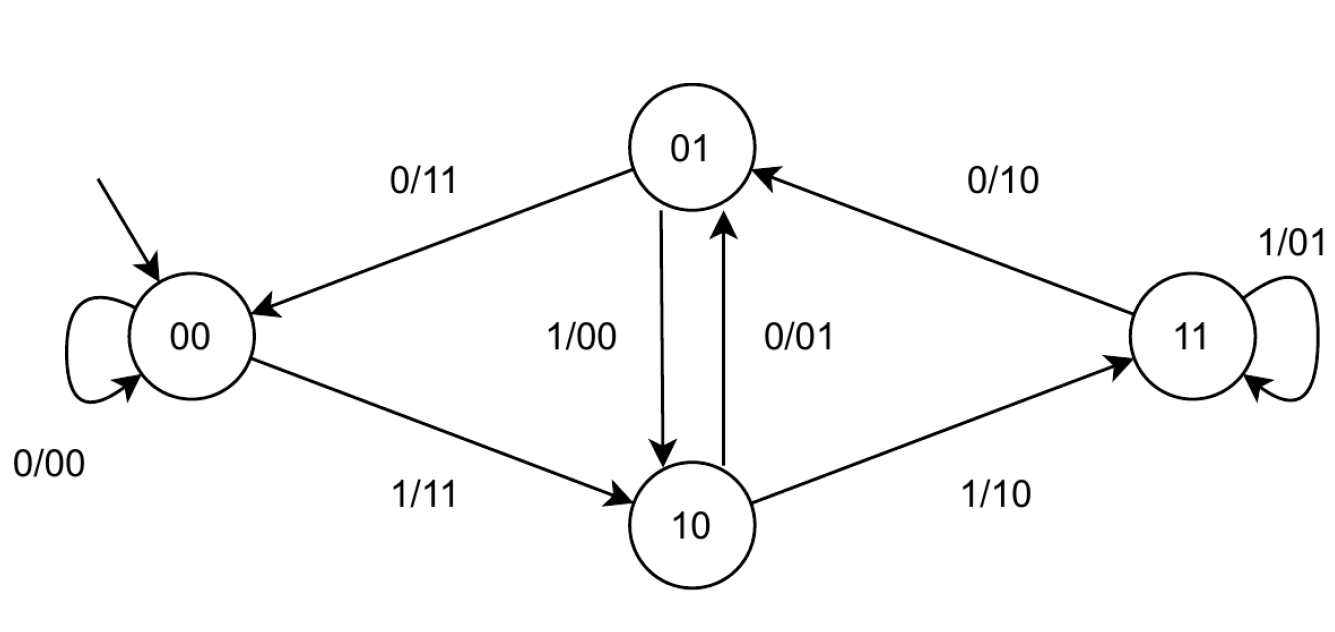
\includegraphics[width=1\textwidth]{conv_mealy}
    \caption{Convolutore}
    \label{fig:conv_mealy}
\end{figure}
Il suo stato iniziale, che è anche quello al quale si torna dopo aver ricevuto un segnale di \verb^RESET^, è lo stato \verb^00^.
Concatenando i 2 bit di uscita, si crea un flusso continuo Y da 1 bit, che sarà lungo $8*W*2$.
Va sottolineato che il convolutore non viene riportato allo stato \verb^00^ all'inizio di ogni parola, ma solo quando riceve un segnale di \verb^RESET^.

\subsubsection{Esempio di codifica}
Applicando, ad esempio, il codice convoluzionale $\frac{1}{2}$ al numero binario \verb^01011101^, si avrebbe la seguente situazione:
\begin{table}[H]
    \centering
    \begin{tabular}{ c | c c c c c c c c } 
    \hline
    \verb^k^ & 0 & 1 & 2 & 3 & 4 & 5 & 6 & 7 \\
    \hline
    $U_{\small{k}}$ & 0 & 1 & 0 & 1 & 1 & 1 & 0 & 1 \\
    $p_{\small{1k}}$ & 0 & 1 & 0 & 0 & 1 & 0 & 1 & 0 \\
    $p_{\small{2k}}$ & 0 & 1 & 1 & 0 & 0 & 1 & 0 & 0 \\
    next state & 00 & 10 & 01 & 10 & 11 & 11 & 01 & 10 \\
    \end{tabular}
    \caption{Applicazione del codice convoluzionale al numero \verb^01011101^}
\end{table}
I 2 byte in uscita saranno: \verb^00110100^ e \verb^10011000^.

\subsection{Parallelizzazione}
Scopo della parallelizzazione (o deserializzazione) dei bit è quello di tornare ad avere un flusso di parole da 8 bit ciascuna da poter scrivere in memoria.
Ogni byte di Y rappresenta quindi una parola che farà parte del risultato finale, costituito complessivamente da $2*W$ parole.

\subsection{Dati e rappresentazione in memoria}
Ogni parola (da 8 bit) può essere letta dalla memoria tramite indirizzamento al byte nel quale essa è memorizzata.
Il byte all'indirizzo \verb^0^ rappresenta la lunghezza della sequenza da codificare, le cui parole si trovano tra l'indirizzo \verb^1^ e \verb^999^.
Dall'indirizzo \verb^1000^ in poi sono invece contenuti i byte della sequenza di uscita.

\begin{center}
    \renewcommand{\arraystretch}{2}
    \definecolor{Gray}{gray}{0.95}
    \newcolumntype{g}{>{\columncolor{Gray}}m{15em}}
    \begin{tabular}{ | g | i }
        \cline{0-0}
        Lunghezza input (W) & Indirizzo 0\\
        \cline{0-0}
        \tikzmark[xshift=-10pt,yshift=2ex]{x}Byte 1 da codificare & Indirizzo 1\\
        \cline{0-0}
        Byte 2 da codificare & Indirizzo 2\\
        \cline{0-0}
        ... & \\
        \cline{0-0}
        \tikzmark[xshift=-10pt,yshift=-1.5ex]{y}Byte W da codificare & Indirizzo W\\
        \cline{0-0}
        ... & \\
        \cline{0-0}
        \tikzmark[xshift=-10pt,yshift=2ex]{w}Byte 1 in uscita & Indirizzo 1000\\
        \cline{0-0}
        Byte 2 in uscita & Indirizzo 1001\\
        \cline{0-0}
        ... & \\
        \cline{0-0}
        Byte 2W-1 in uscita & Indirizzo 1000+2W-2\\
        \cline{0-0}
        \tikzmark[xshift=-10pt,yshift=-1.5ex]{z}Byte 2W in uscita & Indirizzo 1000+2W-1\\
        \cline{0-0}
        ... & \\
    \end{tabular}
    \hspace{-4,5cm}
    \drawbrace[brace mirrored, thick]{x}{y}
    \drawbrace[brace mirrored, thick]{w}{z}
    \annote[left]{brace-1}{Sequenza in input}
    \annote[left]{brace-2}{Sequenza in uscita}
\end{center}

Poiché la lunghezza della sequenza di ingresso è rappresentata in binario su 8 bit, e poiché per codificare un numero decimale \verb^n^ in binario occorrono $log_{\small{2}}n$ bit, il massimo numero di byte da codificare è dato da $2^8-1$, quindi \verb^255^.
Come conseguenza, gli indirizzi di memoria da \verb^256^ a \verb^999^ rimarranno sempre inutilizzati.

\subsection{Funzionamento}
Per prima cosa, il componente legge il byte all'indirizzo di memoria \verb^0^, che rappresenta la lunghezza della sequenza di ingresso (W).
Quindi passa all'indirizzo \verb^1^, nel quale è contenuta la prima parola da codificare. 
La parola viene serializzata e ogni bit passa attraverso il convolutore.
I 2 bit in uscita dal convolutore vengono concatenati ad ogni iterazione, ed in seguito alla loro parallelizzazione, si scrivono i 2 byte in uscita agli indirizzi \verb^1000^ e \verb^1001^. 
Dunque si passa a leggere la seconda parola da codificare, finché non si raggiunge la W-esima parola, i cui  byte di uscita corrispondenti saranno scritti agli indirizzi \verb^1000+2W-2^ e \verb^1000+2W-1^.

\subsubsection{Esempio di funzionamento}
Un esempio del funzionamento completo del modulo, nel caso in cui il flusso in input sia costituito da 2 sole parole, è descritto nelle seguenti tabelle.
\begin{table}[H]
\renewcommand{\arraystretch}{1.5}
\parbox{.45\linewidth}{
    \centering
    \begin{tabular}{ | i | c | }
    \hline
    Indirizzo & Contenuto \\
    \hline
    \verb^0^ & \verb^00000010^ \\
    \hline
    \verb^1^ & \verb^01011101^ \\
    \hline
    \verb^2^ & \verb^11000110^ \\
    \hline
    ... & ... \\
    \hline
    \verb^1000^ & ... \\
    \hline
    \verb^1001^ & ... \\
    \hline
    \verb^1002^ & ... \\
    \hline
    \verb^1003^ & ... \\
    \hline
    ... & ... \\
    \hline
    \end{tabular}
    \vspace{0,3cm}
    \caption{Stato iniziale memoria}
}
\parbox{.45\linewidth}{
    \centering
    \begin{tabular}{ | i | c | } 
    \hline
    Indirizzo & Contenuto \\
    \hline
    \verb^0^ & \verb^00000010^ \\
    \hline
    \verb^1^ & \verb^01011101^ \\
    \hline
    \verb^2^ & \verb^11000110^ \\
    \hline
    ... & ... \\
    \hline
    \verb^1000^ & \verb^00110100^ \\
    \hline
    \verb^1001^ & \verb^10011000^ \\
    \hline
    \verb^1002^ & \verb^10011011^ \\
    \hline
    \verb^1003^ & \verb^00111010^ \\
    \hline
    ... & ... \\
    \hline
    \end{tabular}
    \vspace{0,3cm}
    \caption{Stato finale memoria}
}
\end{table}
In particolare è stato messo in evidenza lo stato della memoria prima e dopo l'elaborazione.
Per quanto riguarda la codifica, si faccia sempre riferimento alla Tabella 1.


%%%%%%%%%%%%%%%%%%%%%%%%%%%%
%%%%%%% ARCHITETTURA %%%%%%%
%%%%%%%%%%%%%%%%%%%%%%%%%%%%
\newpage
\section{Architettura}
\subsection{Interfaccia del componente}
L'interfaccia del componente è la seguente:
\begin{lstlisting}[language=VHDL]
entity project_reti_logiche is
    port (
        i_clk : in std_logic;
        i_rst : in std_logic;
        i_start : in std_logic;
        i_data : in std_logic_vector(7 downto 0);
        o_address : out std_logic_vector(15 downto 0);
        o_done : out std_logic;
        o_en : out std_logic;
        o_we : out std_logic;
        o_data : out std_logic_vector (7 downto 0)
    );
end project_reti_logiche;
\end{lstlisting}
\vspace{0.3cm}
Più nello specifico:
\begin{itemize}
  \item[\verb^i\_clk^] è il segnale di \verb^CLOCK^;
  \item[\verb^i\_rst^] è il segnale di \verb^RESET^ (inizializza la macchina a dei valori di default);
  \item[\verb^i\_start^] è il segnale di \verb^START^;
  \item[\verb^i\_data^] è il segnale che arriva in seguito ad una richiesta di lettura dalla memoria;
  \item[\verb^o\_address^] è il segnale che trasmette l'indirizzo alla memoria;
  \item[\verb^o\_done^] è il segnale di uscita che determina la fine dell'eleborazione;
  \item[\verb^o\_en^] è il segnale di \verb^ENABLE^ da mandare alla memoria per poter leggere o scrivere;
  \item[\verb^o\_we^] è il segnale di \verb^WRITE ENABLE^ da mandare alla memoria con valore \verb^1^ se si vuole scrivere e \verb^0^ se si vuole leggere da essa;
  \item[\verb^o\_data^] è il segnale di uscita verso la memoria.
\end{itemize}

\subsubsection{Inizio e fine computazione}
Il modulo inizia l'elaborazione nel momento in cui assume valore \verb^1^ il segnale \verb^i_start^, che rimane alto.
Dopo aver scritto l'intero risultato in memoria, anche il segnale \verb^o_done^ viene portato ad \verb^1^, per comunicare il termine della computazione.
Questo segnale rimane alto finché \verb^i_start^ non torna a \verb^0^.
Dal momento in cui anche \verb^o_done^ viene riportato al valore logico basso, può avere inizio un'altra computazione, seguendo le stesse modalità.
Un segnale di \verb^RESET^ precede sempre la prima computazione, e se \verb^i_rst^ dovesse valere \verb^1^ in qualche momento durante l'elaborazione, i segnali dovranno essere portati ai loro valori di default.

\subsection{Macchina a stati}
Si è deciso di implementare il componente tramite una macchina a stati finiti, la cui rappresentazione è la seguente:
\begin{figure}[H]
    \centering
    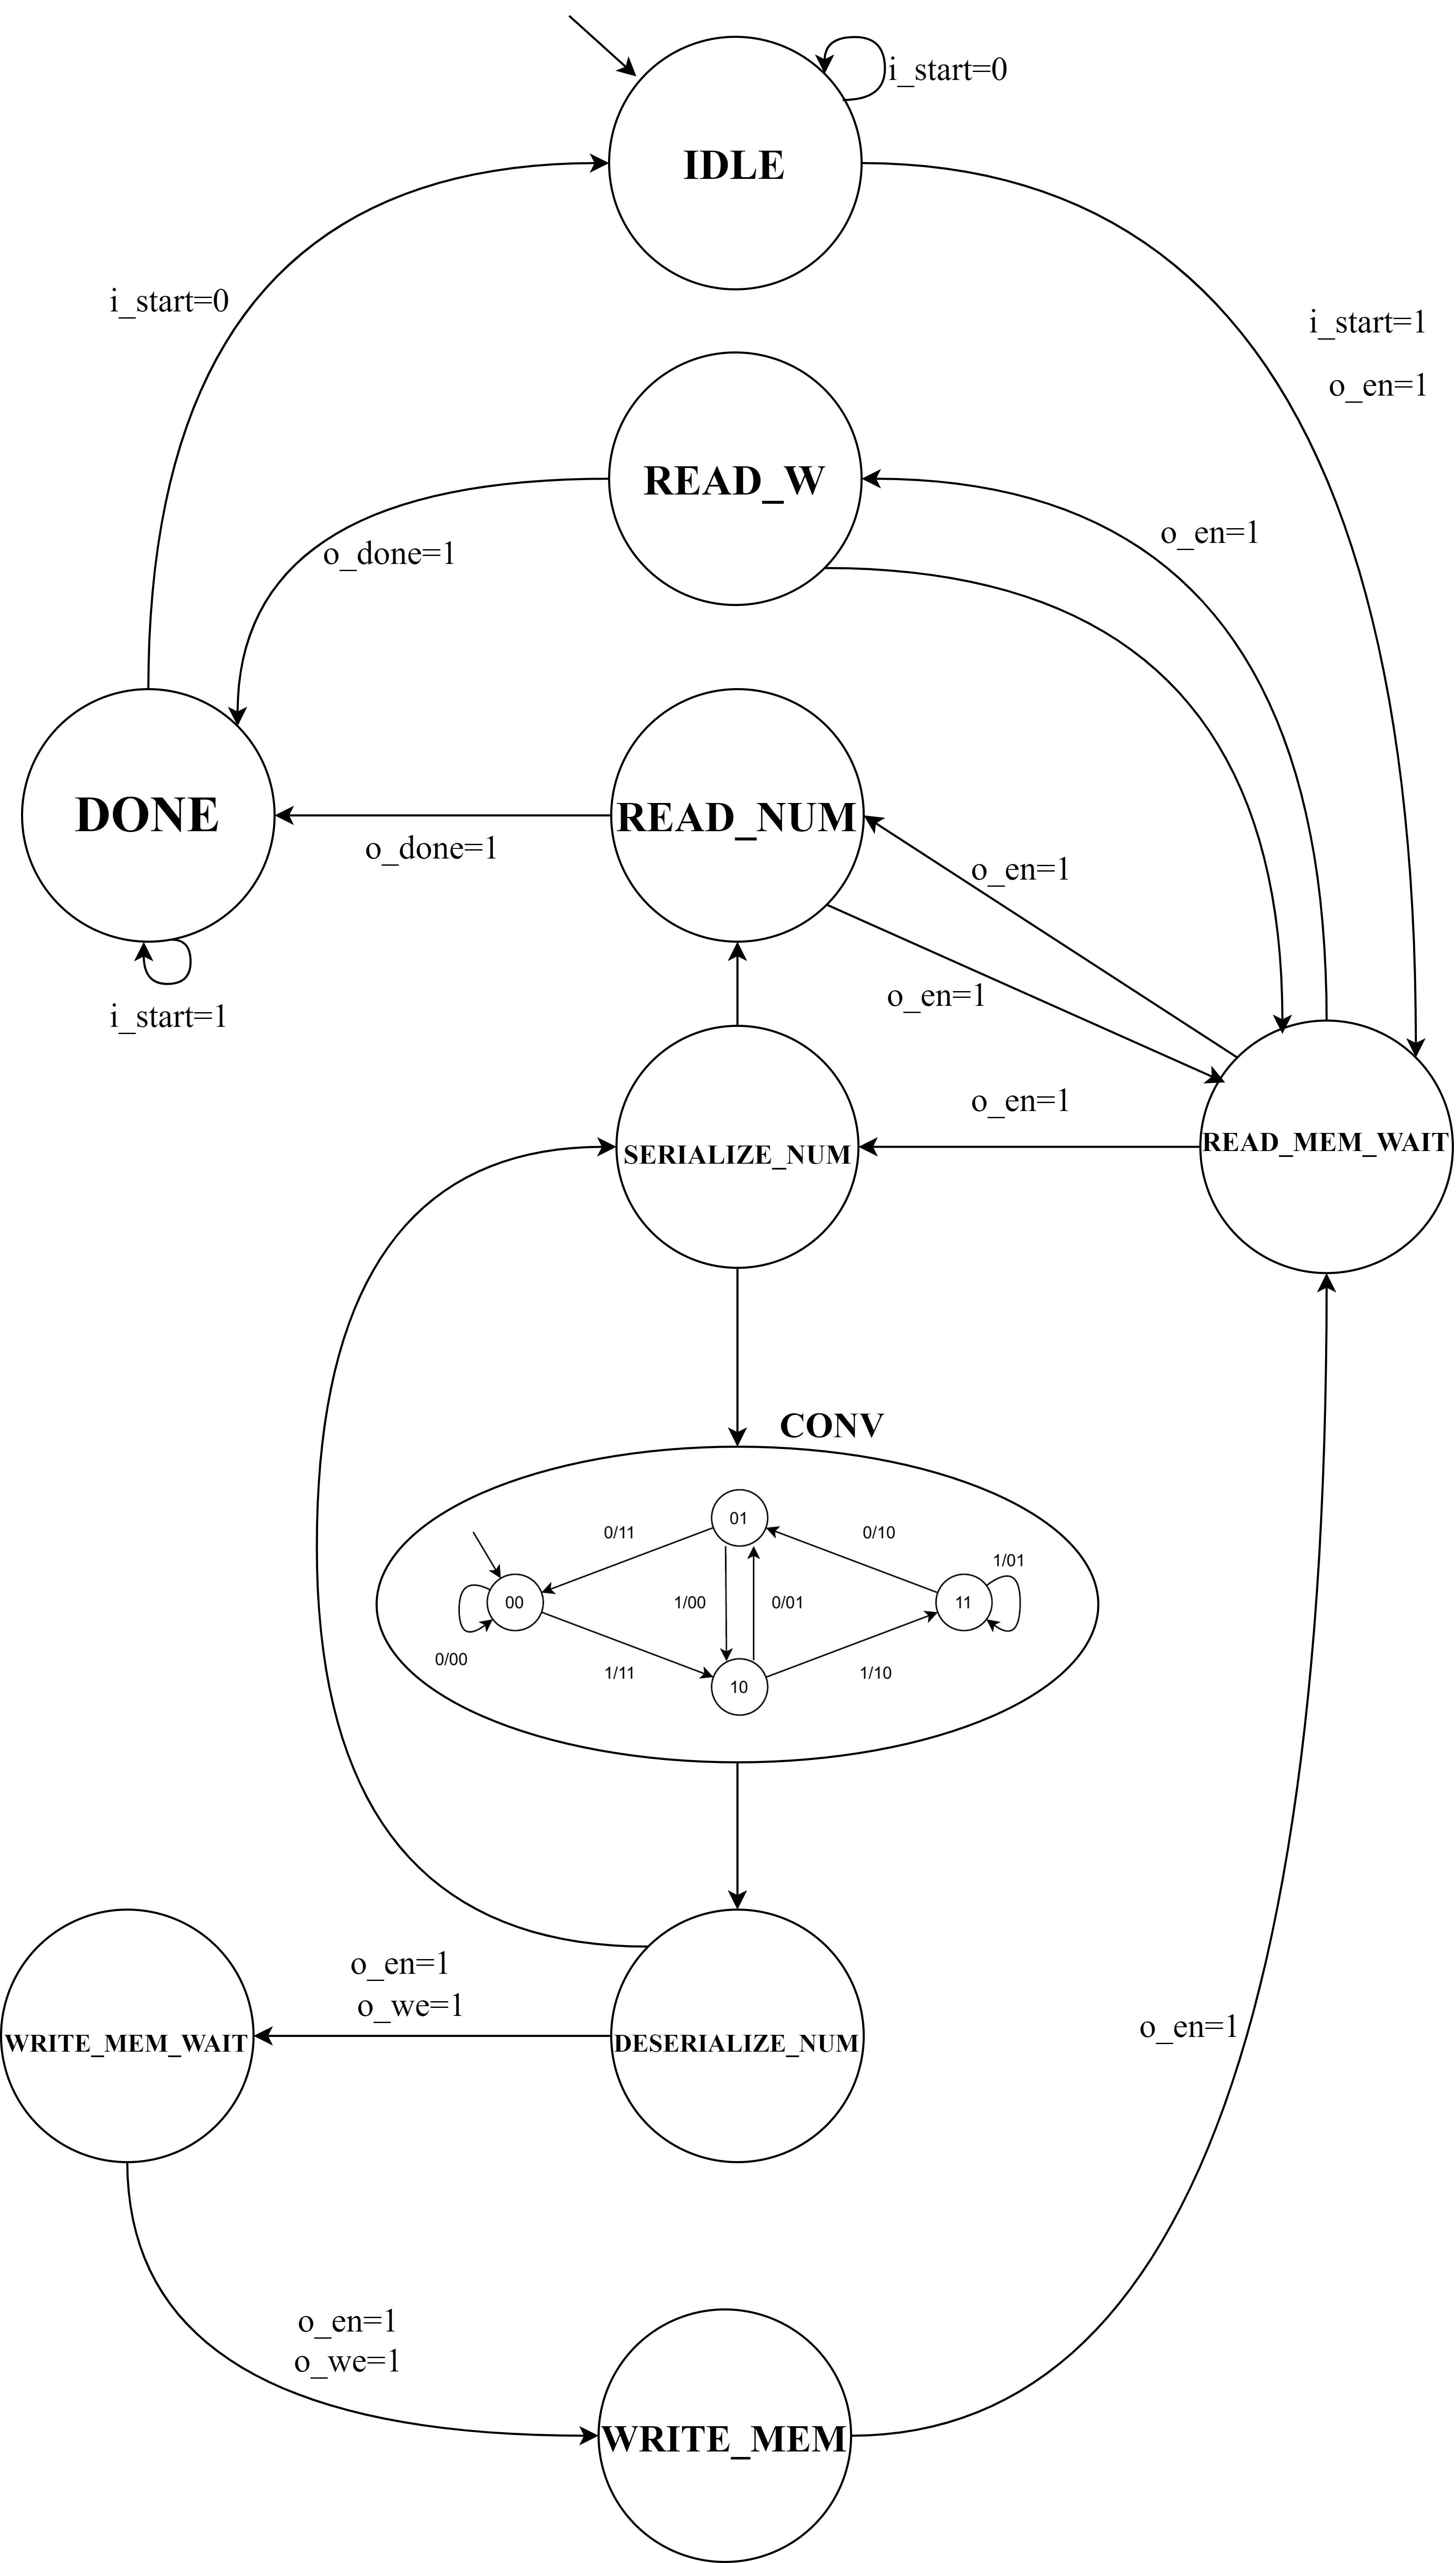
\includegraphics[width=0.7\textwidth]{fsm}
    \caption{Macchina a stati finiti}
    \label{fig:fsm}
\end{figure}
Non è esplicitato il fatto che ad ogni ciclo di clock i segnali \verb^o_done^, \verb^o_en^ e \verb^o_we^ vengono messi a \verb^0^. Inoltre da ogni stato si torna ad \verb^IDLE^ se \verb^i_rst^ vale \verb^1^.
\newpage
Di seguito è fornita una breve descrizione per ognuno dei 10 stati di cui si compone la FSM.
\begin{itemize}
    \item[\verb^IDLE^]: stato iniziale, nel quale viene riportata la macchina in caso di \verb^RESET^ o di terminazione della sequenza
    \item[\verb^READ\_MEM\_WAIT^]: stato di attesa necessario affinché avvenga il corretto aggiornamento dei dati provenienti dalla memoria
    \item[\verb^READ\_W^]: stato nel quale viene letto il numero di parole che compongono la sequenza da codificare
    \item[\verb^READ\_NUM^]: stato nel quale viene letta la parola da codificare
    \item[\verb^SERIALIZE\_NUM^]: stato nel quale vengono serializzati i bit della parola letta nello stato \verb^READ_NUM^
    \item[\verb^CONV^]: contiene un'altra macchina a stati finiti che rappresenta il convolutore. I suoi stati sono: \verb^S_00^, \verb^S_01^, \verb^S_10^, \verb^S_11^, come mostrato nella Figura 3
    \item[\verb^DESERIALIZE\_NUM^]: stato nel quale vengono deserializzati i bit provenienti dal convolutore
    \item[\verb^WRITE\_MEM\_WAIT^]: stato di attesa necessario affinché si possano scrivere correttamente i dati in memoria
    \item[\verb^WRITE\_MEM^]: stato nel quale avviene l'effettiva scrittura dei dati, e l'aggiornamento dell'indirizzo della memoria per l'operazione successiva
    \item[\verb^DONE^]: stato per la terminazione della computazione di una sequenza. Si rimane in questo stato fin quando \verb^i_start^ non torna a \verb^0^, dopodiché si torna allo stato iniziale
\end{itemize}

\subsubsection{Scelte implementative}
L'intero componente è stato realizzato utilizzando due soli processi: \verb^state_reg^ e \verb^cod_conv^.
\begin{itemize}
    \item[\verb^state\_reg^]: processo che gestisce gli aggiornamenti dei segnali ad ogni ciclo di clock e la routine di \verb^RESET^
    \item[\verb^cod\_conv^]: processo in cui è descritto il funzionamento del componente e dei vari stati della FSM
\end{itemize}
Come accennato precedentemente, lo stato \verb^CONV^, che rappresenta il convolutore, è a sua volta una macchina a stati. Dal codice VHDL abbiamo infatti:
\begin{lstlisting}[language=VHDL]
type state_type is (IDLE, READ_W, READ_NUM, READ_MEM_WAIT, 
    SERIALIZE_NUM, CONV, DESERIALIZE_NUM, WRITE_MEM_WAIT, 
    WRITE_MEM, DONE);
type state_type_conv is (S_00, S_01, S_10, S_11);
\end{lstlisting}
Si è optato per questa soluzione per mantenere il concetto di codificatore convoluzionale come macchina a stati a sé, rendendo la notazione più compatta ed evitando l'introduzione di altri 4 (o più) stati nella FSM principale.

\subsection{Segnali interni}
\begin{itemize}
    \item[\verb^current\_state^]: segnale che rappresenta lo stato corrente della macchina a stati finiti (Figura 3). Il suo valore di default è \verb^IDLE^
    \item[\verb^conv\_current\_state^]: segnale che rappresenta lo stato corrente del convolutore, all'interno dello stato \verb^CONV^ della FSM principale. Il suo valore di default è \verb^S_00^
    \item[\verb^return\_state^]: segnale che tiene traccia dello stato successivo di \verb^READ_MEM_WAIT^. Il suo valore di default è \verb^IDLE^
    \item[\verb^o\_address\_copy^]: segnale che tiene memoria del valore di \verb^o_address^. Il suo valore di default è \verb^(others => '0')^
    \item[\verb^words\_number^]: segnale che rappresenta il numero di parole della sequenza. Il suo valore di default è \verb^0^
    \item[\verb^count\_read^]: segnale che tiene conto del numero di parole già lette della sequenza. Il suo valore di default è \verb^0^
    \item[\verb^count\_write^]: segnale che tiene conto del numero di parole scritte in memoria. Il suo valore di default è \verb^0^
    \item[\verb^i^]: contatore utile per la serializzazione della parola letta. Il suo valore iniziale è \verb^7^, e viene decrementato di 1 ogni volta che avviene la serializzazione di un bit. Una volta completata la serializzazione di una parola, viene riportato a \verb^7^
    \item[\verb^signal\_out^]: segnale che contiene l'i-esimo bit della parola letta, serializzato. Il suo valore di default è \verb^0^
    \item[\verb^j^]: contatore utile per la deserializzazione. Il suo valore iniziale è \verb^7^, e viene decrementato di 2 ogni volta che vengono deserializzati due bit. Viene riportato a \verb^7^ dopo la scrittura di una parola in memoria
    \item[\verb^new\_out\_1^]: segnale che contiene il primo bit in uscita dal convolutore. Il suo valore di default è \verb^0^
    \item[\verb^new\_out\_2^]: segnale che contiene il secondo bit in uscita dal convolutore. Il suo valore di default è \verb^0^
    \item[\verb^new\_number^]: segnale che rappresenta la parola da scrivere in memoria. Il suo valore di default è \verb^(others => '0')^
\end{itemize}

\vspace{0,6cm}
Sono stati aggiunti inoltre dei segnali, denotati con suffisso \verb^_next^, in abbinamento alla maggior parte dei segnali appena descritti. L'obiettivo è quello di evitare la sintesi di latch. I segnali di tipo \verb^_next^ aggiornano i relativi segnali ad ogni ciclo di clock.


%%%%%%%%%%%%%%%%%%%%%%%%%%%%%%%%%%%%%%%%%%%%%%%%
%%%%%%% RISULTATI SPERIMENTALI - SINTESI %%%%%%%
%%%%%%%%%%%%%%%%%%%%%%%%%%%%%%%%%%%%%%%%%%%%%%%%
\newpage
\section{Risultati sperimentali - Sintesi}
In questa sezione sono riportate le informazioni più rilevanti raccolte durante la fase di sintesi.
\subsection{Utilization}
Nella stesura del codice VHDL si è cercato di ottimizzare in modo da mantenere al minimo l'area occupata dal componente, e al contempo evitarne comportamenti indesiderati.
\\Il componente risulta essere sintetizzabile e implementabile in modo corretto, con 103 LUT e 73 Flip Flop.
Quanto si evince dal \emph{Report Utilization} inserito qui di seguito, è innanzitutto il fatto che le percentuali di LUT e Flip Flop inferiti durante la sintesi sono entrambe inferiori all'1\%.
Dunque, come auspicato, solo una minima parte di tutta disponibilità dell'FPGA è effettivamente utilizzata.
\\In aggiunta, durante la sintesi non sono inferiti latch, situazione che impedisce propagazioni non volute di segnali.

\begin{center}
\verb|+-------------------------+------+-------+-----------+-------+|\nopagebreak\\
\verb=|        Site Type        | Used | Fixed | Available | Util% |=\nopagebreak\\
\verb=+-------------------------+------+-------+-----------+-------+=\nopagebreak\\
\verb=| Slice LUTs*             |  103 |     0 |    134600 |  0.08 |=\nopagebreak\\
\verb=|   LUT as Logic          |  103 |     0 |    134600 |  0.08 |=\nopagebreak\\
\verb=|   LUT as Memory         |    0 |     0 |     46200 |  0.00 |=\nopagebreak\\
\verb=| Slice Registers         |   73 |     0 |    269200 |  0.03 |=\nopagebreak\\
\verb=|   Register as Flip Flop |   73 |     0 |    269200 |  0.03 |=\nopagebreak\\
\verb=|   Register as Latch     |    0 |     0 |    269200 |  0.00 |=\nopagebreak\\
\verb=| F7 Muxes                |    0 |     0 |     67300 |  0.00 |=\nopagebreak\\
\verb=| F8 Muxes                |    0 |     0 |     33650 |  0.00 |=\nopagebreak\\
\verb|+-------------------------+------+-------+-----------+-------+|\nopagebreak\\
\end{center}

\subsection{Timing}
Dalle specifiche, il componente deve essere in grado di operare con un periodo di clock $T_{\small{clk}} \le 100ns$. Per verificare questo, è stato aggiunto un timing constraint con $T_{\small{clk}} = 100ns$ e duty cycle pari al 50\%.
Analizzando il \emph{Report Timing Summary} in Figura 4, è chiaro che questa condizione è rispettata.
\\
A livello teorico,
\begin{center}
    $T_{\small{clk, min}} = T_{\small{clk}} - WNS$
\end{center}
\\dove WNS è il Worst Negative Slack.
\\Imponendo vincoli sempre più stringenti sul periodo del clock, è stato constatato che $T_{\small{clk}} = 4ns$ è il minimo periodo per il quale il componente continua a funzionare correttamente.
È possibile avere conferma di questo dalla Figura 5, nella quale il WNS è ancora positivo.

\begin{figure}[H]
    \centering
    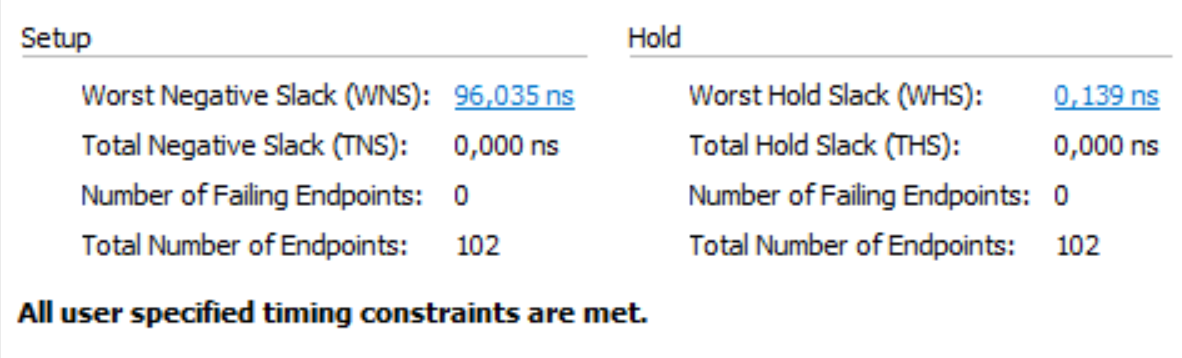
\includegraphics[width=1\textwidth]{report_timing_summary_100ns}
    \caption{\emph{Report Timing Summary ($T_{\small{clk}} = 100 ns$)}}
    \label{fig:timing100}
\end{figure}

\begin{figure}[h]
    \centering
    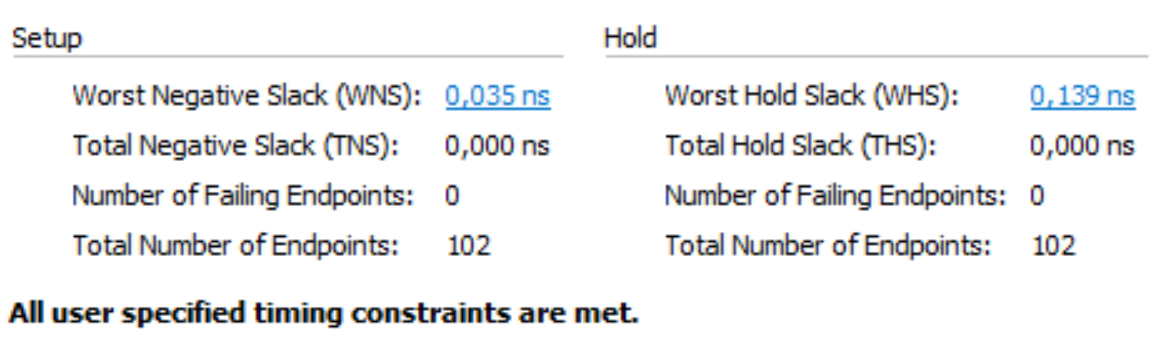
\includegraphics[width=1\textwidth]{report_timing_summary_4ns}
    \caption{\emph{Report Timing Summary $T_{\small{clk}} = 4 ns$}}
    \label{fig:timing4}
\end{figure}


%%%%%%%%%%%%%%%%%%%%%%%%%%%%%%%%%%%%%%%%%%%%%%%%%%%%
%%%%%%% RISULTATI SPERIMENTALI - SIMULAZIONI %%%%%%%
%%%%%%%%%%%%%%%%%%%%%%%%%%%%%%%%%%%%%%%%%%%%%%%%%%%%
\newpage
\section{Risultati sperimentali - Simulazioni}
Dopo la stesura del codice, questo è stato sottoposto ai testbench forniti insieme alle specifiche, al fine di accertare che il modulo operasse correttamente.
\\In particolare il focus è stato posto su:
\begin{enumerate}
    \item casi limite;
    \item funzionamento del \verb^RESET^;
    \item codifica continua;
    \item stress test.
\end{enumerate}

\vspace{0,3cm}
Nelle successive immagini si nota che il valore del segnale di uscita dalla RAM, prima di essere utilizzato, e quindi prima di essere aggiornato al valore corretto, subisce delle variazioni.
Queste però non influiscono sul giusto funzionamento del componente.

\subsection{Test casi limite}
\subsubsection{Minimo}
Viene testato il caso limite in cui il numero di parole da codificare è uguale a 0.\\
Risultati delle simulazioni:
\begin{itemize}
    \item \emph{Behavioral}: 850 000 ps
    \item \emph{Post Synthesis}: 850 100  ps
\end{itemize}

\begin{figure}[H]
    \centering
    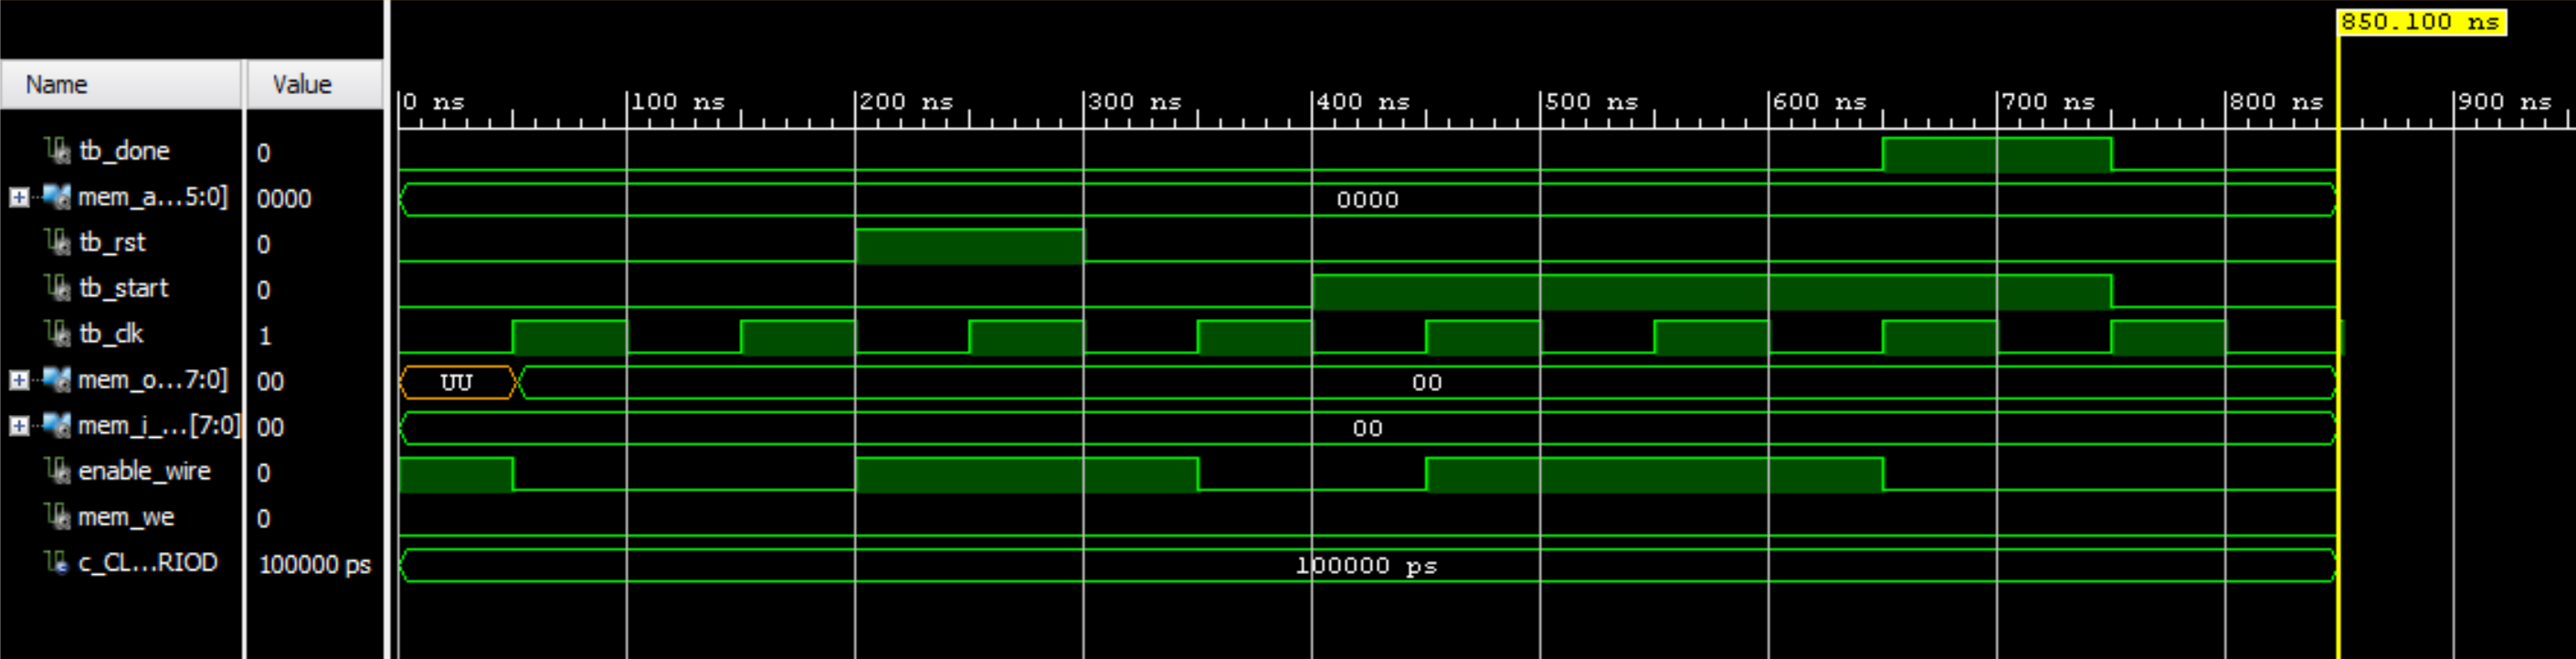
\includegraphics[width=1.2\textwidth, height=0.2\textheight]{test_min}
    \caption{Simulazione \emph{Post Synthesis} - minima sequenza in ingresso}
    \label{fig:min}
\end{figure}

\subsubsection{Massimo}
È testato il caso limite in cui il numero di parole da codificare è massimo, e quindi pari a 255.\\
Risultati delle simulazioni:
\begin{itemize}
    \item \emph{Behavioral}: 842 550 000  ps
    \item \emph{Post Synthesis}: 842 550 100 ps
\end{itemize}

\begin{figure}[h]
    \centering
    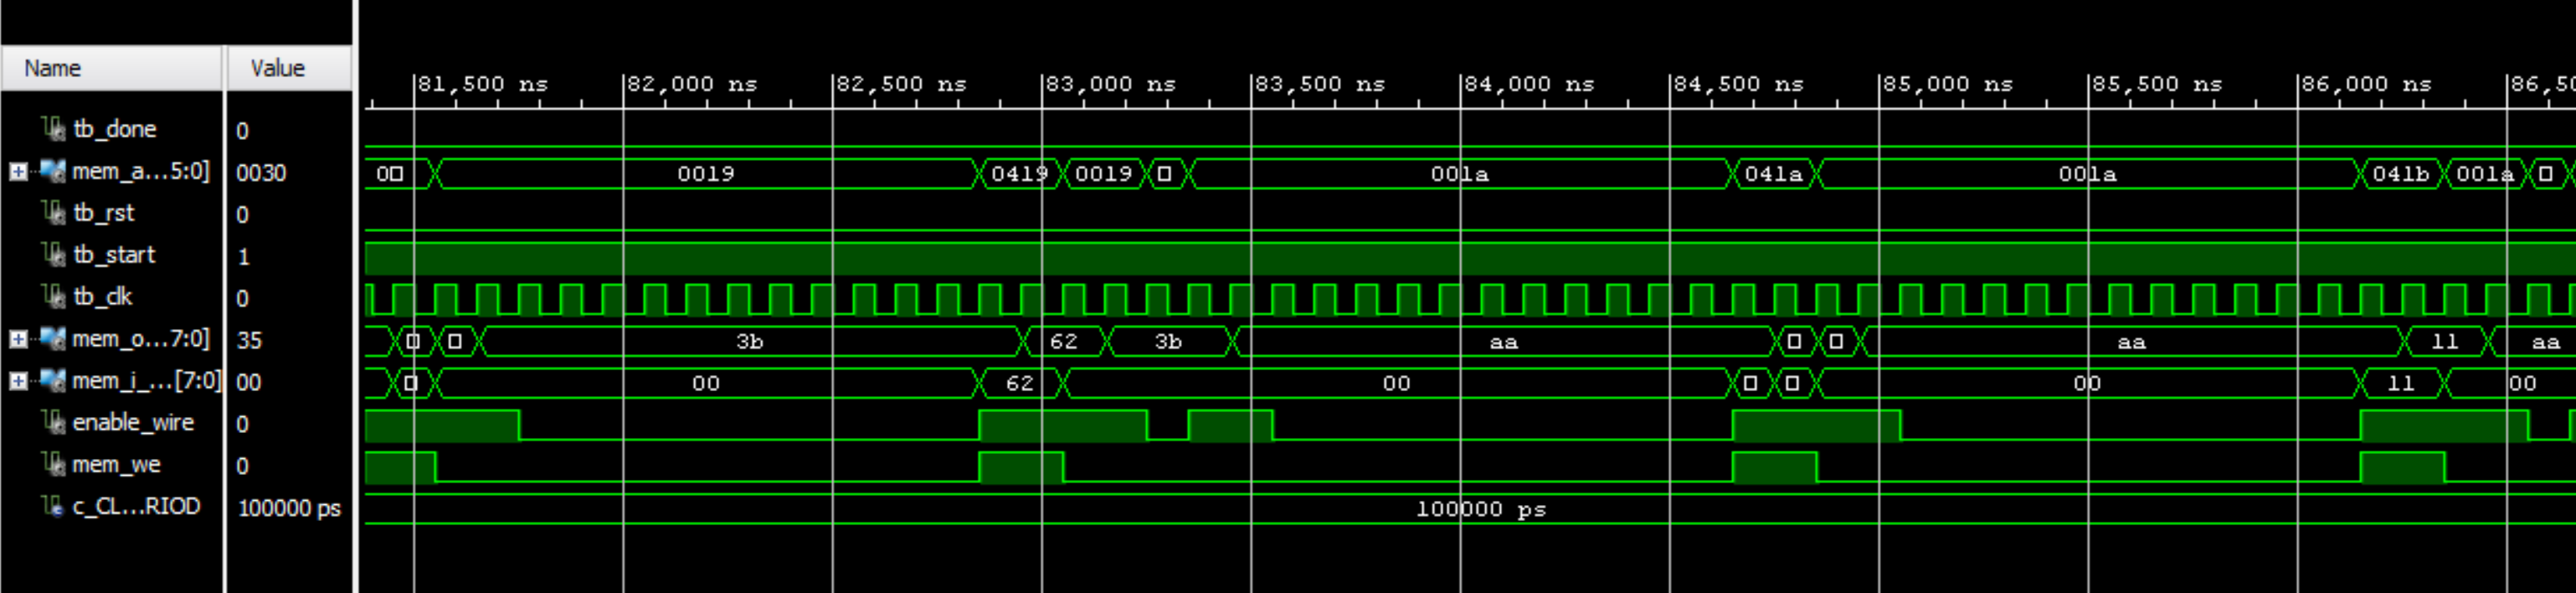
\includegraphics[width=1.2\textwidth, height=0.2\textheight]{test_max}
    \caption{Simulazione \emph{Post Synthesis} - massima sequenza in ingresso}
    \label{fig:max}
\end{figure}

\newpage
\subsection{Test reset}
In questo test viene effettuato un \verb^RESET^ asincrono.\\
Risultati delle simulazioni:
\begin{itemize}
    \item \emph{Behavioral}: 22 750 000 ps
    \item \emph{Post Synthesis}: 22 750 100 ps
\end{itemize}
\begin{figure}[h]
    \centering
    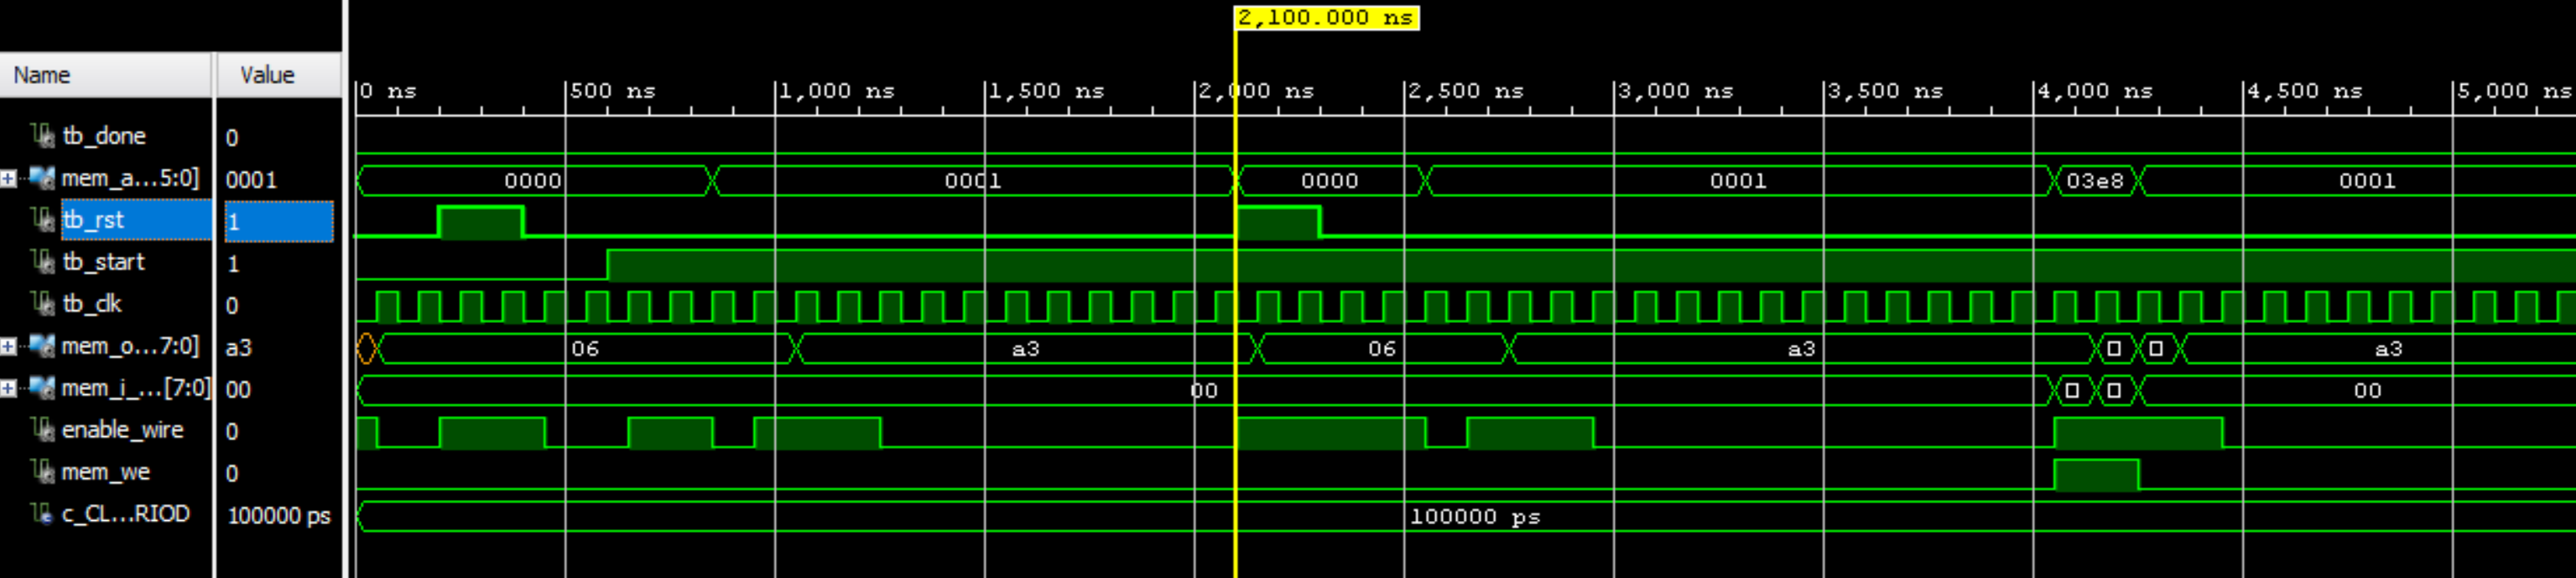
\includegraphics[width=1.2\textwidth, height=0.2\textheight]{test_reset}
    \caption{Simulazione \emph{Post Synthesis} - funzionamento del \verb^RESET^}
    \label{fig:reset}
\end{figure}


\subsection{Test codifica continua}
Tre sequenze sono codificate di seguito, senza ricezione del segnale di \verb^RESET^ tra l'una e l'altra.\\
Risultati delle simulazioni:
\begin{itemize}
    \item \emph{Behavioral}: 52 350 000 ps
    \item \emph{Post Synthesis}: 52 350 100 ps
\end{itemize}

\newpage

\begin{figure}[H]
    \centering
    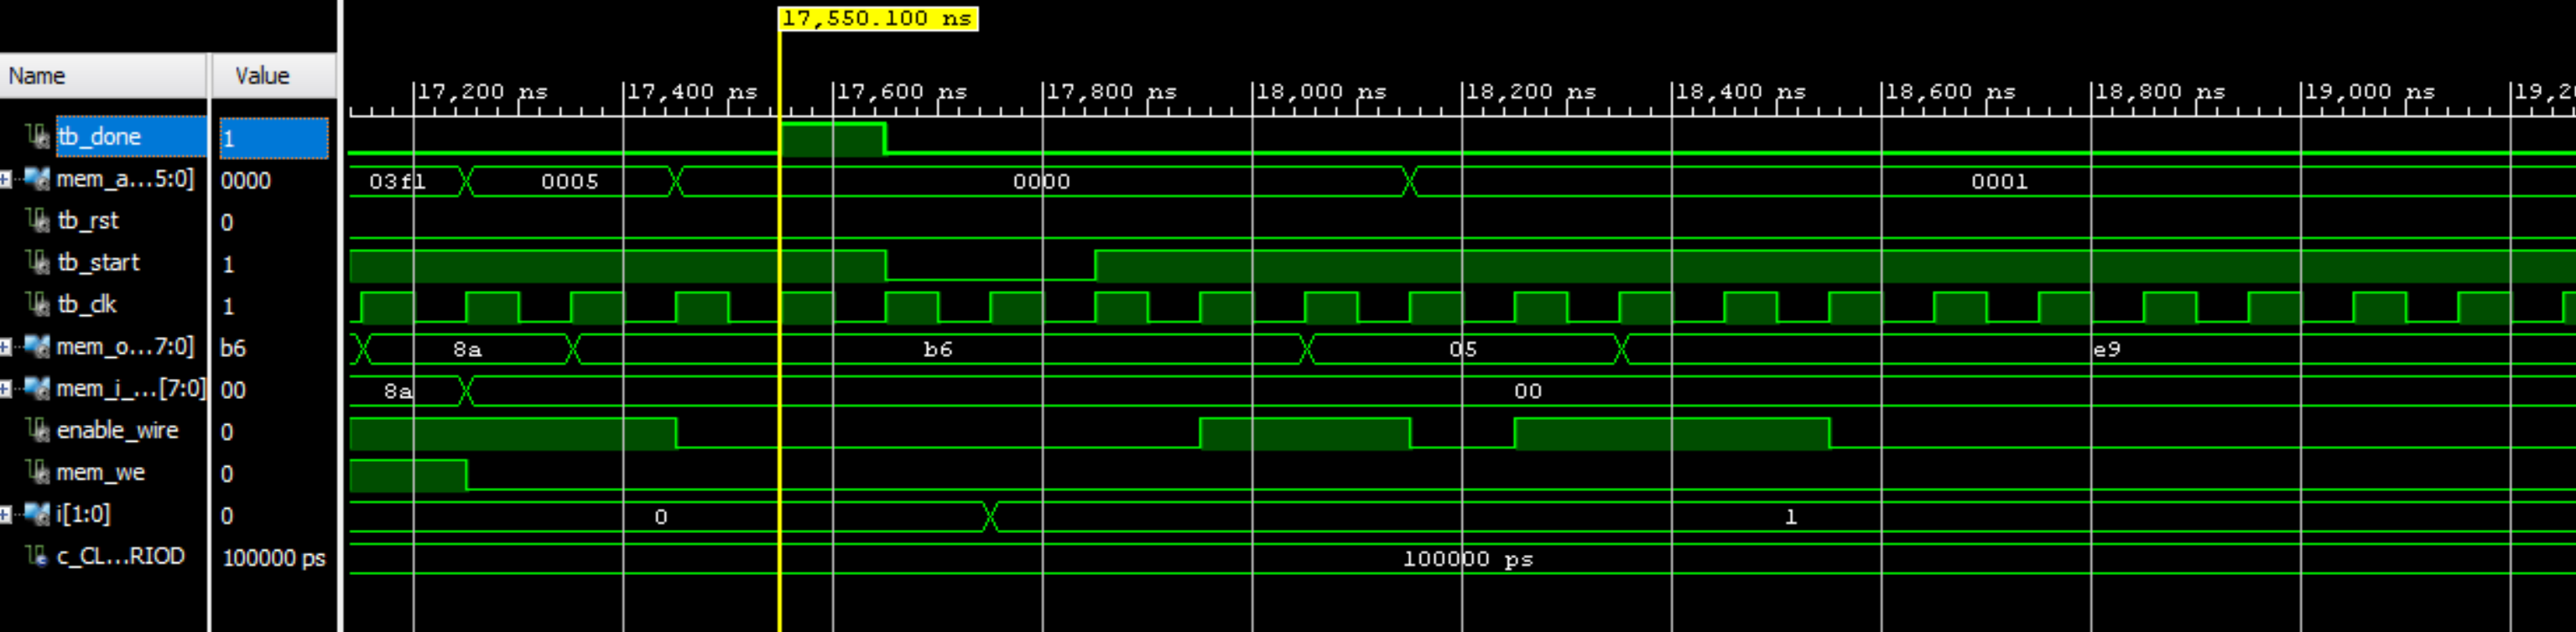
\includegraphics[width=1.2\textwidth, height=0.2\textheight]{test_codcont}
    \caption{Simulazione \emph{Post Synthesis} - codifica continua}
    \label{fig:codcont}
\end{figure}

\subsection{Stress test}
Il componente è stato sottoposto anche ad uno stress test creato utilizzando un generatore di test casuali scritto in Python, che prevedeva circa 4000 sequenze composte da un numero di parole variabile, compreso tra 0 e 255.


%%%%%%%%%%%%%%%%%%%%%%%%%%%
%%%%%%% CONCLUSIONI %%%%%%%
%%%%%%%%%%%%%%%%%%%%%%%%%%%
\vspace{2cm}
\section{Conclusioni}
Una prima versione del codice prevedeva che il segnale \verb^o_en^, che permette la comunicazione con la memoria, rimanesse sempre ad \verb^1^, e che da ogni stato si passasse sempre attraverso uno stato di wait prima di raggiungere il successivo.
Successive fasi di ottimizzazione hanno fatto in modo che \verb^o_en^ venisse portato ad \verb^1^ solo quando necessario, e che si evitassero inutili passaggi attraverso stati di wait, riducendo notevolmente anche i tempi di elaborazione.
Si è cercato di ridurre al minimo l'utilizzo di LUT e Flip Flop, nonché di stati della FSM e segnali interni.
Tutti i test eseguiti hanno avuto esito positivo, sia in \emph{Behavioral} che in \emph{Post Synthesis}.
\\Dunque il componente risulta essere in grado di applicare il codice convoluzionale $\frac{1}{2}$ a qualsiasi sequenza in ingresso, operando in maniera conforme alle specifiche.

\end{document}